
\documentclass[ms.tex]{subfiles}
\begin{document}

\section{Galactic Properties}
\label{sec:galprops}

\begin{figure*}
\centering
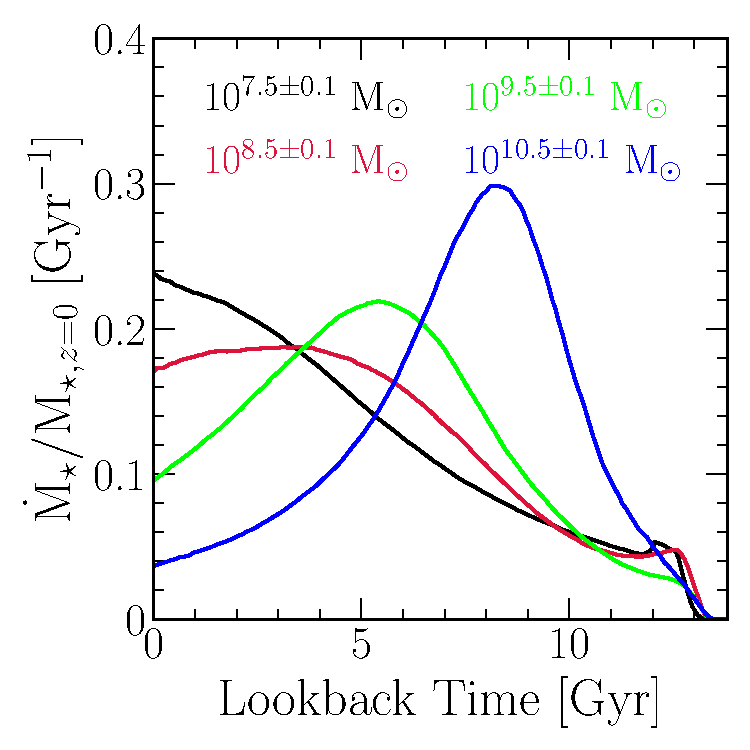
\includegraphics[scale = 0.43]{umachine_sfhs.pdf}
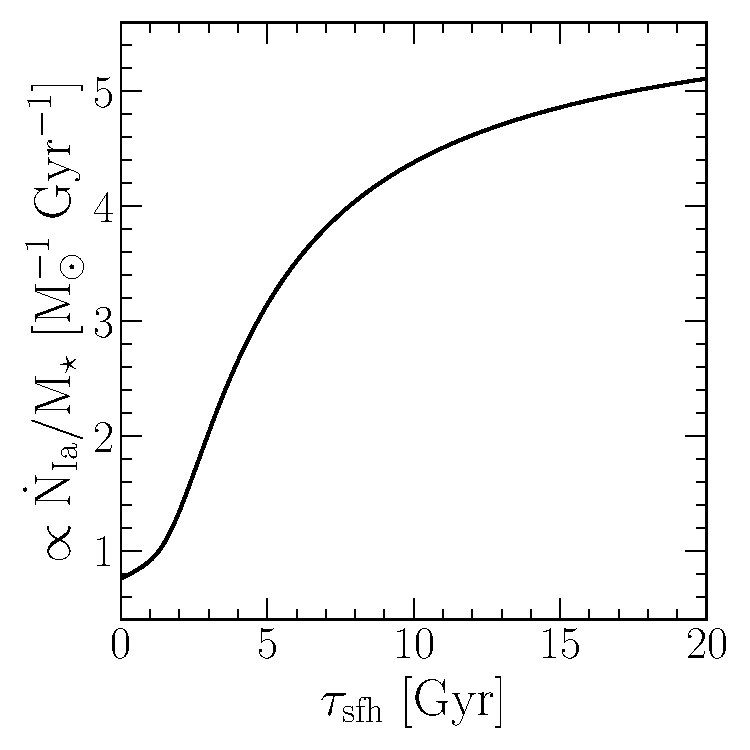
\includegraphics[scale = 0.42]{iarate_vs_tausfh.pdf}
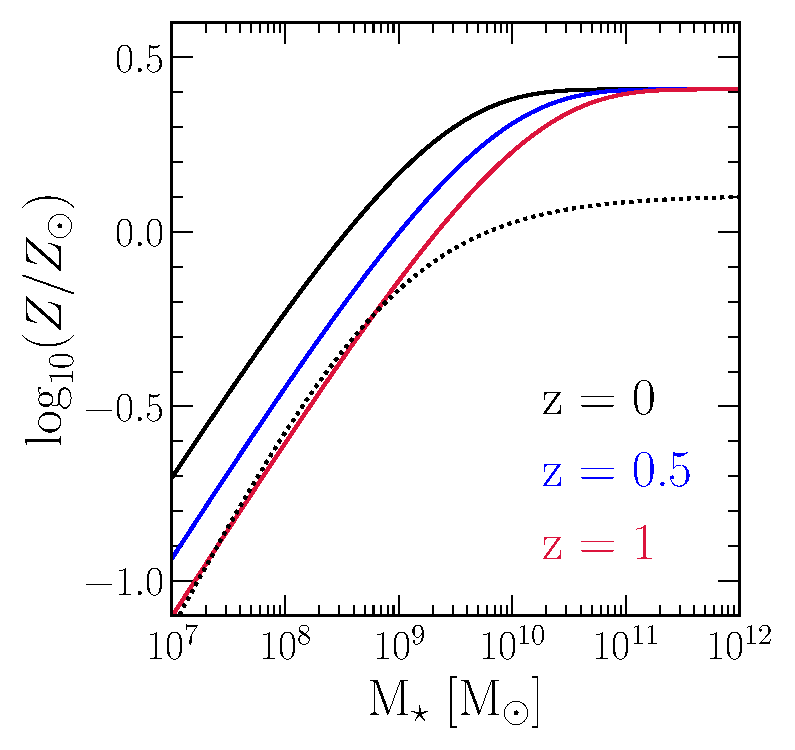
\includegraphics[scale = 0.42]{mzr.pdf}
\caption{
\textbf{Left}: The best-fit mean SFH of galaxies with present-day stellar
masses of $\mstar = 10^{7.5 \pm 0.1}$ (black),~$10^{8.5 \pm 0.1}$ (red),
$10^{9.5 \pm 0.1}$ (green), and $10^{10.5 \pm 0.1} \msun$ (blue) as reported
by~\um~and normalized by the present-day stellar mass itself.
\textbf{Middle}: The specific SN Ia rate as a function of the e-folding
timescale of the SFH~$\tau_\text{sfh}$ assuming a linear-exponential SFH and a
$\tau^{-1}$ power-law SN Ia DTD.
\textbf{Right}: The redshift-dependent MZR reported by~\citet{Zahid2014} at
$z = 0$ (black solid),~$z = 0.5$ (blue), and~$z = 1$ (red).
For comparison, we additionally plot the MZR measured by
\citet[][black dotted, appropriate for~$z = 0$]{Andrews2013}.
}
\label{fig:sfh_mzr}
\end{figure*}

In this paper, we assume that the strong scaling of the specific SN Ia rate
with stellar mass is due to metallicity effects and conduct simple numerical
calculations to investigate the origin of the effect.
We combine the relationship between galaxy stellar mass and mean SFH and the
popular~$\tau^{-1}$ DTD for SNe Ia~\citep[e.g.][]{Maoz2012a} with empirical
parametrizations of the mass-metallicity relation (MZR) for galaxies
\citep{Tremonti2004, Andrews2013, Zahid2011, Zahid2014}.
Assuming the mean SFH and DTD allows us to compute the characteristic SN Ia
rate for galaxies of a given stellar mass, and by further assuming that the
galaxy lies along the observed MZR, we can simultaneously fold in various
scalings with metallicity~$Z$.
\par
We begin by examining how the mean galactic SFH varies with present-day stellar
mass as predicted by the~\um~semi-analytic model~\citep{Behroozi2019}.
Using dark matter halo properties supplied by the~\textit{Bolshoi-Planck} and
\textit{Multi-Dark Planck 2} dark matter only simulations~\citep{Klypin2016,
Rodriguez-Puebla2016},~\um~follows a convention semi-analytic model framework
(see, e.g., the review in~\citealt{Somerville2015a}) by parametrizing the SFRs
of galaxies as a function of lookback time, the assembly history of the halo,
and the depth of the halo's potential well.
Like other semi-analytic models that came before it,~\um~successfully
reproduces a broad range of well-constrained observables, including stellar
mass functions, cosmic SFRs, specific SFRs, quenched fractions, UV luminosity
functions, and more.
While some semi-analytic models have used the extended Press-Schechter
formalism~\citep{Press1974, Bond1991} to generate halo merger trees and push
the lower stellar mass limit of their model down to~$\mstar \approx 10^7~\msun$
\citep[e.g.][]{Somerville2015b}, an advantage of~\um~is that the high mass
resolution of the~\textit{Bolshoi-Planck} and~\textit{Multi-Dark Planck 2}
simulations allows merger trees down to~$\mstar = 10^{7.2}~\msun$ to be
obtained directly from the simulations.
Dwarf galaxies in this regime are of particular interest to our investigation
because the scaling of the specific SN Ia rate with stellar mass measured by
\citet{Brown2019} extends as low as~$\sim 10^7~\msun$ in their volume-limited
sample and~$\sim 10^6~\msun$ in their full sample.
\par
In the left panel of Fig.~\ref{fig:sfh_mzr}, we plot the best-fit mean SFH as a
function of lookback time in four narrow bins of observed stellar mass taken
from~\um.
In the interest of relating these predictions to data from ASAS-SN
\citep{Shappee2014, Kochanek2017}, an untargeted survey, we take the full
galaxy sample from~\um, including both star forming and quenched galaxies as
well as both centrals and satellites, though centrals are the dominant
population across the full stellar mass range.
In general, low stellar mass galaxies have more extended SFHs than their
higher mass counterparts.
This effect is sufficiently strong such that around~$10^{7.5}~\msun$, typical
SFRs are still increasing at the present day.
In principle, this should impact the characteristic SN Ia rate as a function of
galaxy mass.
\par
Although the details of the SN Ia DTD is a topic of active inquiry
\citep[e.g.][]{Greggio2005, Strolger2020, Freundlich2021}, comparisons of the
cosmic SFH~\citep[e.g.][]{Hopkins2006, Davies2016, Madau2014, Madau2017,
Driver2018} with the volumetric SN Ia rate as a function of redshift suggest
that the cosmic DTD is broadly consistent with a~$\tau^{-1}$ power-law
(\citealp{Maoz2012a};~\citealp*{Maoz2012b};~\citealp{Graur2013, Graur2014}).
A DTD of approximately this form is also expected under the double-degenerate
scenario given population synthesis models of binary white dwarfs and the loss
of angular momentum due to graviational wave emission (e.g.
\citealp{Mennekens2010};~\citealp*{Maoz2014}).
We therefore adopt this parametrization in this paper, though we have
reconducted our analysis using an exponential DTD with a timescale of
$\tau_\text{Ia} = 1.5$ Gyr and found similar results.

\end{document}
